\chapter{Architecture}
\section{Architectural Diagram}
This system has a data-flow architecture (see Figure~\ref{architectualDiagram}) that starts from "Headset" and moves clock-wise to "Audio." This architecture was chosen because there are constant inputs received by the system, and the inputs in general goes through the same route within the system. The data-flow architecture also has build-in concurrency, which can speeds up the process, especially the platform in which the product is embedded.
\begin{figure}
	\centering
    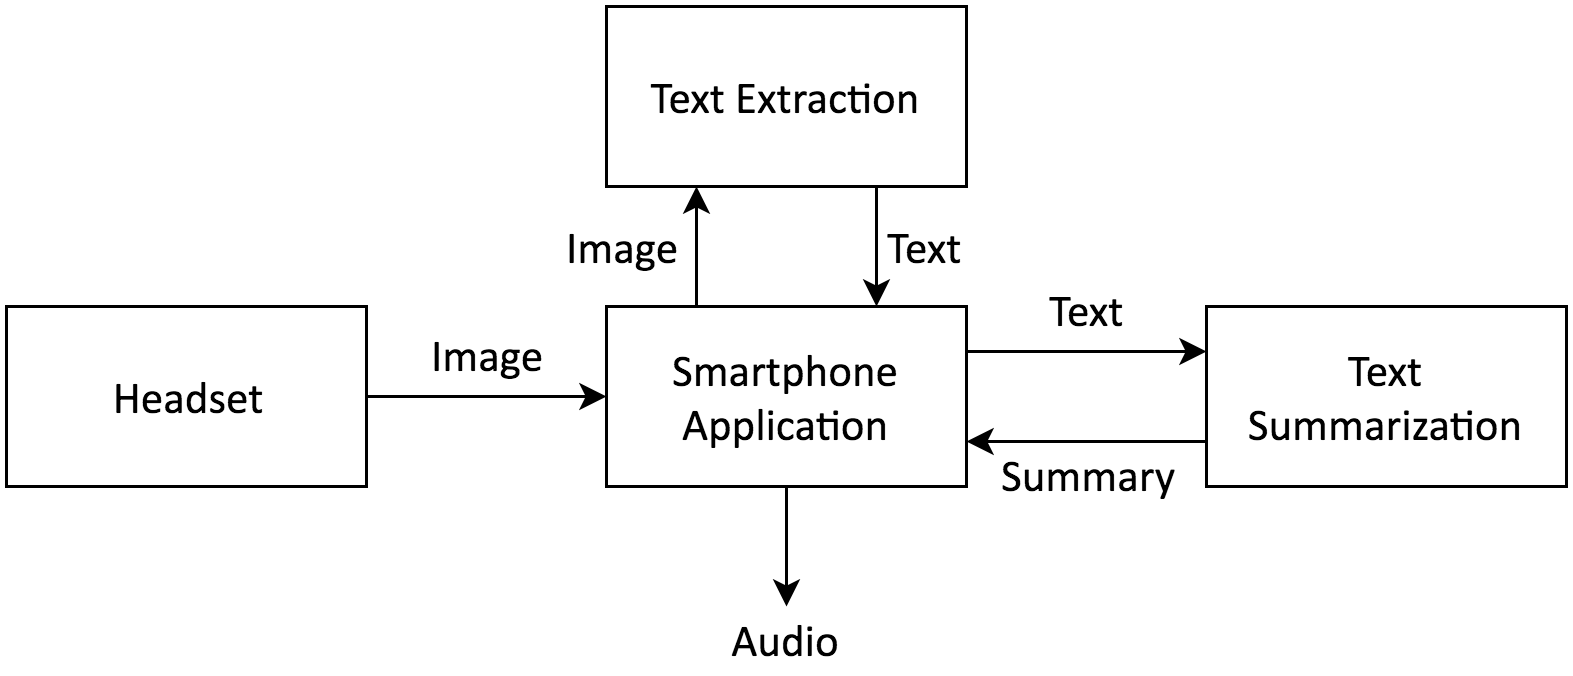
\includegraphics[scale = 0.2]{ArchitectureDiagram.png}
    
    \caption{Architectural Diagram}
	\label{architectualDiagram}
\end{figure}

\section{Hardware Interface}
PRAHVI, itself, is a wearable headset device that attaches to a typical pair of glasses or can be manufactured as a single assembly. PRAHVI is comprised of a Raspberry Pi Zero compute board coupled with a standard Raspberry Pi Camera.

The modular nature of these parts allows for future expansion and easy repairs for the user and for other developers. The Raspberry Pi Zero, in particular, was chosen for its low power consumption and wide application flexibility. Once the device is connected to the user's smartphone and the accompanying app is opened, PRAHVI powers up and immediately begins communicating with the smartphone.

\section{User Interface}
The user interface of PRAHVI is mainly comprised of a gesture pad that allows for text translation and navigation with minimal use of visual and audible cues. Once the user connects the headset and opens the app, PRAHVI immediately begins scanning the environment, adjusting the camera parameters to find a set point that produces a clear, usable image. Swiping the gesture area allows the user to navigate the text in realtime, with the smartphone providing haptic feedback. Tapping the gesture area starts the translation process, as PRAHVI captures an image and sends the image to the backend, before signaling to the user a quick summary (see Text Summarization section for more information) of the text and then a full translation.

\section{Backend}
The backend of PRAHVI is a flask web application. It exposes all the functionality related to the computer vision, optical character recognition, and text summary into a an easy web inteface for our iPhone application to use.

The interface of the backend is a simple set of HTTP endpoints which are summarized as follows:

\begin{table}[]
\centering
\caption{My caption}
\label{my-label}
\begin{tabular}{|l|l|l|l|l|}
\hline
\multicolumn{1}{|c|}{Endpoint}                  & \multicolumn{1}{c|}{Input}               & \multicolumn{1}{c|}{Output}                & \multicolumn{1}{c|}{HTTP METHOD} & \multicolumn{1}{c|}{Description}                                                   \\ \hline
\textlessdomain\textgreater/api/v1/image/ocr3   & File: Image                              & JSON: \{ result: string \}                 & POST                             & Prahvi's image to text algorithm using tesseract 3                                 \\ \hline
\textlessdomain\textgreater/api/v1/image/ocr4   & File: Image                              & JSON: \{ result: string \}                 & POST                             & Prahvi's image to text algorithm using tesseract 4                                 \\ \hline
\textlessdomain\textgreater/api/v1/text/tfidf   & String                                   & JSON: \{ result: \{ term: score, ... \} \} & POST                             & Takes in a document string and outputs the scores of all the terms in the document \\ \hline
\textlessdomain\textgreater/api/v1/text/compare & JSON: \{ text1: string, text2: string \} & JSON: \{ result: int{[}0, 1{]} \}          & POST                             & Returns a score of how similar the documents are.                                  \\ \hline
\end{tabular}
\end{table}



\begin{itemize}

\item Originally, all of the functionality listed above was implemented within the iPhone application, however due to the limited compute resources of the iPhone, PRAHVI's requirements were not being met. Image to text translation on average would take half a min, and the iPhone architecture was mangling some of the text results. For these reasons, these functionalities have been moved the backend end hosted on a server allows for a faster processing time as noted in our testbench. The server is a linux machine running an Intel(R) Core(TM) i7-4900MQ CPU @ 2.80GHz multi-core processor.

\end{itemize}

\section{System Flow}
Once the camera captures the image and sends the image to the smart phone, the image will pass through the pre-processing stage to detect whether the image will be processed or not. Once the image passes the pre-processing stage, it is processed for text, and is then output as audio feedback.

\section{Text Extraction}

\subsection{Image Pre-processing}
When the smart phone application receives the image, the image is then passed through 2 filters. The first filter detects the blurriness of the image. If the image is blurred, the phone will reject the image because it is hard to extract useful information from a blurred imaged. If the image passed the blurriness test, it will then be used to compare to the previous detected image for similarity. If the image is similar (or the same), the image will also be rejected, because the information from the same document is stored in the device from the previous capture. These 2 filters help to improve the efficiency of the system and save time waited by the user.

\subsubsection{Blurriness Test}
To test for blurriness, variance of Laplacian is used. The image is treated as a 2-dimensional matrix, and the variance of Laplacian of the matrix is generated. The variance of Laplacian of the image is then compared to a threshold value (the threshold value used for this system is 50). If the variance of Laplacian of the image is lower than the threshold, then the image is blurred, otherwise, it is not.

\subsubsection{Similarity Test}
The similarity test uses the accelerated-KAZE (AKAZE) local features matching.\footnote{http://docs.opencv.org/3.0-beta/doc/tutorials/features2d/akaze\_matching/akaze\_matching.html}~The AKAZE local features matching returns a list of matches between the two images. If the number of matches is above the threshold (the threshold value used for this system is 1000), then the images is said to be similar.

\subsection{Image Processing}
\begin{figure}
	\centering
    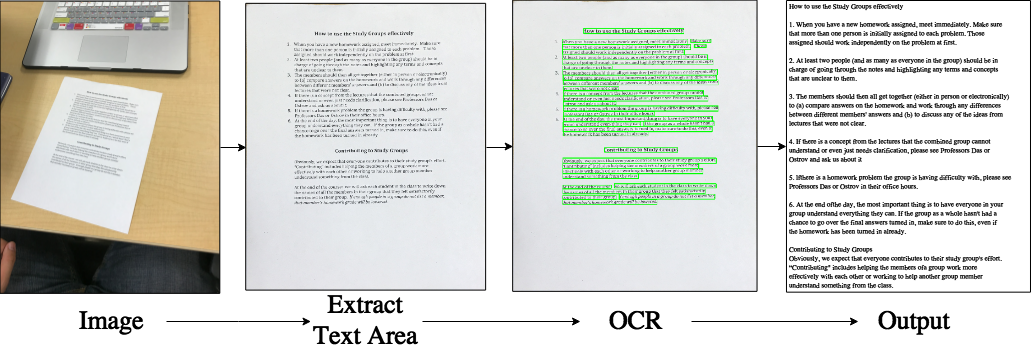
\includegraphics[scale = 0.4]{ImageProcess.png}
    
    \caption{Image Process Flow}
	\label{imageProcessFlow}
\end{figure}
When the image passed the blurriness test and the similarity test, the system will try to detect the text area in the image and extract the text area. The extracted text area is then sent to the Tesseract Optical Character Recognition (OCR) Engine to convert the image to computer encoded characters. (see Figure~\ref{imageProcessFlow})

\pagebreak

\subsubsection{Text Area Extraction}
To extract the text area, a copy of the image is first blurred (Gaussian Blur is used in implementation) to detect the edges in the image (Canny Edge Detection is used in implementation). From the edges of the image, contours are then collected and sorted in descending order based on their area.


From the list of sorted contours, the biggest contour that can be approximated to a quadrilateral is identified as the text area. The text area is then applied with a perspective transformation to convert the text area to a rectangle	 as if the document is scanned. This increases the accuracy of the result from Tesseract OCR Engine. 

\subsubsection{Text Detection}
The transformed text area is processed by the Tesseract OCR Engine to identify the bounding boxes of the text in the image and convert the image to computer encoded characters. The computer-encoded characters are then processed to extract key features and feedback to the user.

\section{Text Summarization}
In order to provide users with a summary of the extracted text we use an algorithm called Term Frequency-Inverse Document Frequency. (TFIDF) The reason why TFIDF was chosen for our text summary is because it's one of the more popular and well known term-weighting schemes, it's easy to implement, and once it's set up it is computationally fast.

The goals of TFIDF are to obtain statistically important keywords from a text article. 

It does this by giving each word in the target document a score based on two statistics, the word frequency and the inverse document frequency.

The word frequency is simply the number of times the word appears in the target document and the inverse document frequency is calculated by taking the log of the total number of documents in a text corpus (described below) divided by the number of documents that the word appears in.

The final score for each word is calculated as follows: 
$tf(t, d) * idf(t, D)$  
where,
$tf(t, d) = 1$ if term $t$	is in Document $d$ else it's $0$
$idf(t, D) = log(\frac{N}{|d \in D : t \in d|}$
where,
$N$ is the number of documents in the corpus $N = |D|$
${|d \in D : t \in d|}$: number of documents where the term $t$ appears 

The rationale behind the TFIDF algorithm is to reduce the importance of words that appear often yet have no overall significance. Examples of such words are: the, and, is, etc.


The corpus of documents are gathered in the news domain so that our text summarization is inline with the domain of PRAHVI functional requirements. Our strategy was to build our corpus by scraping the top online news repositories for all of there news articles. 

We took the 50 top online news websites. We used a Python library called Newspaper to gather the content of every article currently exists on the site.

Once our corpus was collected we precomputed the inverse document frequencies for each term in our corpus.
